\subsection{www.unsw.edu}

Con el fin de probar la herramienta implementada para este trabajo, y analizar el funcionamiento del Z-Score como medida para hallar nodos distinguidos dentro de una red, se envió un paquete ICMP con destino al sitio web de la University of New South Wales, ubicada en australia. El experimento se realizó dentro de los laboratorios de la facultad, al igual que los siguientes que se presentarán en este trabajo práctico, en consecuencia esperamos que el calculo del puntaje nos permita discernir al menos un salto de mayor importancia con respecto a los otros, por ejemplo un salto transoceánico. En primer lugar podemos observar el recorrido realizado por el paquete en el siguiente mapa:

\begin{figure}[H]
  \centering	
	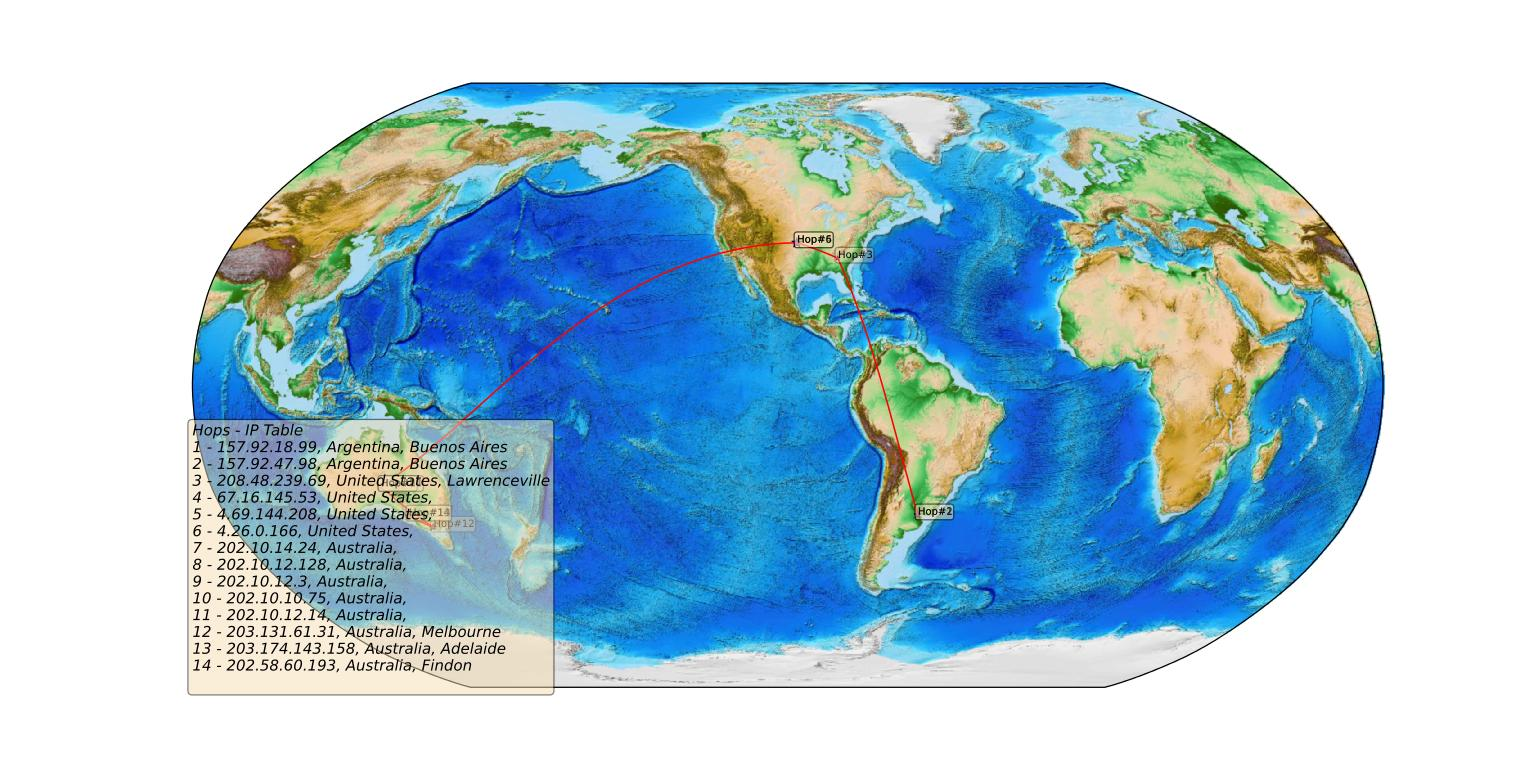
\includegraphics[scale=0.3]{../australia-experiment/figure_1.jpeg}
  \caption{Planisferio el viaje realizado por el paquete resaltado en rojo.}
	\label{fig:histo-src-sitiotrabajo}
\end{figure}

Como se puede observar se halla un salto de los Estados Unidos a Australia entre el sexto y septimo router. Si el Z-Score cumple con su objetivo de la forma esperada, este será resaltado como un \textit{hop} de mayor importancia con respecto a los otros. Veamos que sucede con el \textit{RTT}, que es esperable aumente de manera significativa luego de este salto. El primero del siguiente par de gráficos representa el RTT entre dos host consecutivos, mientras que el segundo representa el acumulado a medida que el paquete se acerca a su destino: 

\begin{figure}[H]
  \centering	
	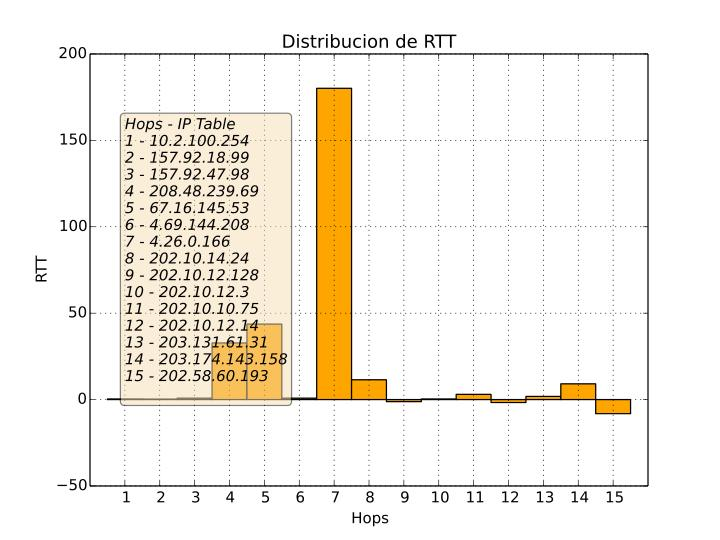
\includegraphics[scale=0.3]{../australia-experiment/bar_rtt.jpeg}
  \caption{RTT entre dos router consecutivos medido en milisegundos.}
	\label{fig:histo-src-sitiotrabajo}
\end{figure}

\begin{figure}[H]
  \centering	
	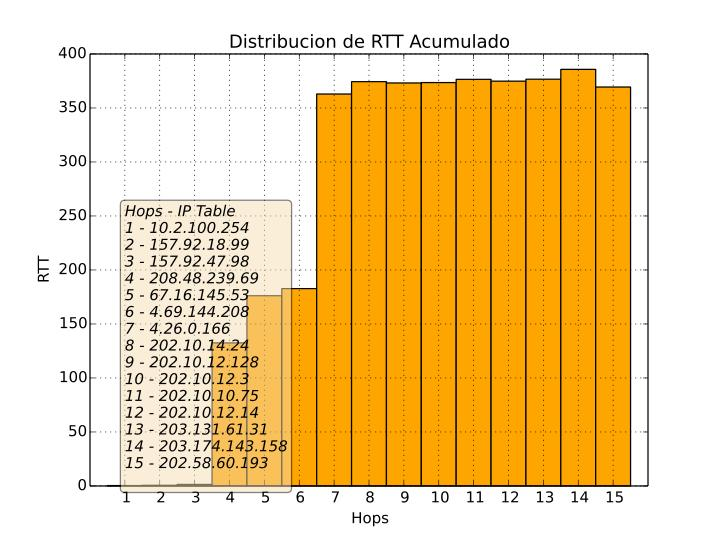
\includegraphics[scale=0.3]{../australia-experiment/bar_rtt_acum.jpeg}
  \caption{RTT acumulado del paquete a medida que avanza en su camino hacia Australia.}
	\label{fig:histo-src-sitiotrabajo}
\end{figure}

Finalmente, presentamos los resultados obtenidos con el Z-Score a partir de los valores obtenidos con la herramienta de \textit{traceroute}. Como se puede ver en el gráfico, la IP distinguida corresponde con el último nodo antes del salto transoceánico con destino a Australia. El resto de los valores o bien son negativos, o no parecen llegar a estar asociados a un nodo representativo del \textit{hop} debido a su reducido puntaje con respecto al mayor de los obtenidos. No se podría afirmar lo mismo en caso de que el puntaje entre varios de los nodos destacados hubiera sido un empate. 

\begin{figure}[H]
  \centering	
	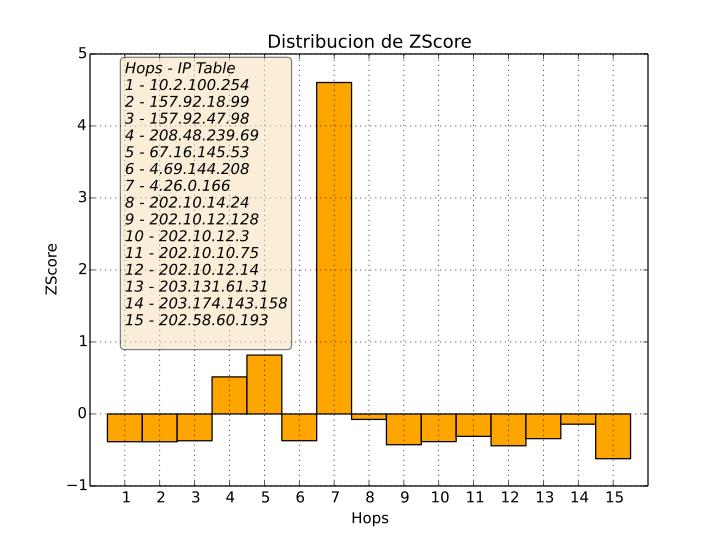
\includegraphics[scale=0.3]{../australia-experiment/bar_z_score.jpeg}
  \caption{Z-Score para cada uno de los saltos.}
	\label{fig:histo-src-sitiotrabajo}
\end{figure}
